%% This is an example first chapter.  You should put chapter/appendix that you
%% write into a separate file, and add a line \include{yourfilename} to
%% main.tex, where `yourfilename.tex' is the name of the chapter/appendix file.
%% You can process specific files by typing their names in at the 
%% \files=
%% prompt when you run the file main.tex through LaTeX.
\chapter{Overview of main procedures}

Finding a practically shortest route on a large road network in a metropolis is not only of algorithmic interests, but also of economic and environmental values. Less travelling time means less fuel consumptions and less carbon emissions. However, finding shortest routes can be challenging, especially when the road traffic is known to be \emph{time-dependent} or \emph{dynamic}, namely, when the road conditions change with respect to time. It may take 10 minutes on average to traverse a particular road at 10a.m, but it is possible that the expected travel time increases to 20 minutes at 5p.m. Moreover, two different roads may have different time-varying patterns. For instance, one road may have a peak traveling time at 12p.m but the other may have two peaks at 8 a.m. and 6 p.m., respectively.

The generalised time-dependent shortest path problem can be formally defined as follows.
\begin{defn}[\emph{Generalised time-dependent shortest path problem}]
In a weighted, directed graph $G=(V,E)$ representing a road network with a weight function $w : E,t \rightarrow \mathbb{R}$, given a source node $u$, a destination node $v$ and a departure time $t$ from $u$, find a path $p$ that satisfies:
\begin{equation}
w(p)=\delta(u,v)=
\begin{cases}
\text{min}\left\{w(p): u\overset{p}{\leadsto}v \right\} &\text{if there is a path from $u$ to $v$,}\\
\infty &\text{otherwise.}
\end{cases}
\end{equation}
where $w(p)$ is the weight of the path $p$ and defined as sum of the weights of its constituent edges, and $\delta(u,v)$ is called the \textbf{shortest-path weight} from $u$ to $v$.
\end{defn}

A typical Bellman-Ford\cite{CLRS09} or Dijkstra's algorithm\cite{Dij59} for finding shortest paths assume the cost of traversing each edge in the abstract graph is constant with respect to time and therefore, do not work on time-de\-pendent road networks without appropriate modifications. Fortunately, most online mapping services such as Google Maps or Apple Maps are able to recommend shortest routes by incorporating real-time traffic information. This project seeks to investigate an alternative approach of finding shortest routes on a dynamic road network based on mining a GPS\footnote{Global Positioning System} trajectory database aggregated from thousands of taxis in Beijing, China.

Chapter two defines several important concepts used in this project. 

Chapter three gives an overview of the GPS-based approach.

Chapter four describes the data pre-processing and presents a novel neural network-based outliner detection method.

Chapter five elaborates the process of building a landmark graph and estimating the expected travel time of each landmark graph edge.

Chapter six introduces the method of evaluating the estimated tralvel time from Chapter five.

\section{Motivations for mining taxi GPS trajectories}
Taxi drivers or any experienced car drivers, more often than not, possess some \emph{implicit} knowledge or intuitions about which route from source $u$ to destination $v$ is the best in terms of travelling time at a particular moment. Such knowledge or intuitions come from everyday experiences. For example, a taxi driver may observe that there are always traffic jams during 6 p.m. to 7 p.m. on a particular street and hence avoids travelling on that street during that period whenever possible. But observations of this kind, albeit valuable, are just too subtle to be captured by any general algorithms and oftentimes, even the drivers themselves may not be aware of that.

However, mining their GPS trajectories can reveal such knowledge to some extent. In a metropolis such as Beijing or New York, taxi drivers are required by regulations to install GPS devices on their cars and to send time-stamped GPS information to a central reporting agency periodically for management and security reasons. Such information typically includes latitudes, longitudes, instantaneous speeds and heading directions. Therefore, the GPS data is readily available and little effort is needed to collect it. By means of mapping to a real road network all GPS data points of a particular taxi during a specific period of time, a GPS trajectory can be obtained to represent the driver's intelligence. 

\section{Practical limitations}
There are some practical limitations that are worth mentioning. 
\subsubsection{Arbitrary sources and destinations}
In a typical map-query use case, a user is able to select an arbitrary source to start with and an arbitrary destination to go to. But this may not be possible in the GPS-based approach, since the taxi GPS trajectories do not necessarily cover every part of a city's map. It is likely that there are no trajectories passing through the source and the destination.
\subsubsection{Low sampling rate}
Taxis report their locations to the central reporting agency at a relatively low rate to conserve energy. For the data set used in this project, the expected sampling interval is one minute. But oftentimes, the GPS device may not be working properly or may be occasionally shut down due to various reasons, which causes the actual sampling interval to fluctuate. 

Even if the sampling interval \emph{is} strictly kept at one minute, for a taxi moving at a typical speed of $60km/h$, it means the distance between two consecutive sample points is $1km$. Such a large distance increases the uncertainty of the \emph{exact} trajectory that the taxi has moved along. The picture\cite{TDR10} below demonstrates a problem caused by low sampling rate and long inter-sample-point distance.
\begin{figure}[h]
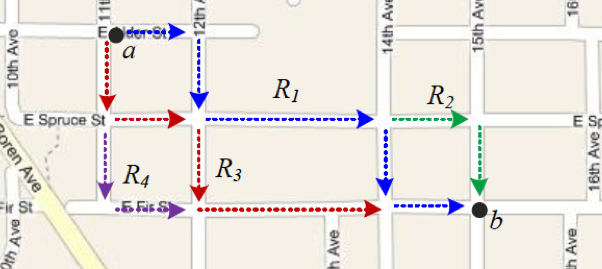
\includegraphics{low_sample_rate}
\centering
\caption{Example of low sampling rate problem}
\end{figure}

The taxi is known to have traversed from point $a$ to point $b$. But there are four possible trajectories from $a$ to $b$. The exact route cannot be determined without additional information in this case.
\subsubsection{Limited GPS accuracy}
After decades of development, the GPS service has achieved great accuracy, but it is still not completely error-free. A report\cite{FP15} in 2015 showed that GPS-enabled smartphones typically have an accuracy of 5 metres \emph{under open sky}. But in a metropolis like Beijing, the actual accuracy may be lower than this value due to the reflection of signals amongst high buildings. Moreover, the data set used in this project was collected in 2009 when GPS devices had lower accuracy than that of today's.

The limited accuracy in GPS devices makes the exact mapping from a GPS data point to a street impossible. In Beijing, there is usually a side road running in parallel with a main road. Due to that limited accuracy, the taxi might be \emph{actually} on the side road but the GPS data point is shown on the main road, or vice versa. 
% This is an example of how you would use tgrind to include an example
% of source code; it is commented out in this template since the code
% example file does not exist.  To use it, you need to remove the '%' on the
% beginning of the line, and insert your own information in the call.
%
%\tagrind[htbp]{code/pmn.s.tex}{Post Multiply Normalization}{opt:pmn}
\section{Related work}
The incentive for carrying out this project comes from a similar project\cite{TDR10}, and similar procedures are followed in this project but with some modifications. 


